\documentclass[document,border=0pt]{standalone}

\usepackage{tikz}
\usepackage{color}
\usetikzlibrary{decorations.pathreplacing}

\begin{document}
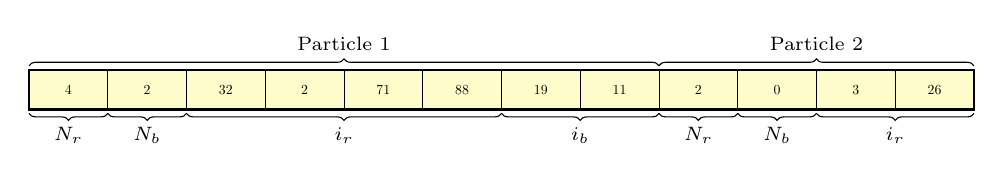
\begin{tikzpicture}

\draw[black, line width=1, fill=yellow!20!white] (0,5.5) rectangle (12, 6.0);
\draw[step=1.0, black, line width=0.25] (0, 5.5) grid (12,  6.0);

\draw (0.5,5.75) node [scale=0.5]{$4$};
\draw (1.5,5.75) node [scale=0.5]{$2$};

\draw (2.5,5.75) node [scale=0.5]{$32$};
\draw (3.5,5.75) node [scale=0.5]{$2$};
\draw (4.5,5.75) node [scale=0.5]{$71$};
\draw (5.5,5.75) node [scale=0.5]{$88$};

\draw (6.5,5.75) node [scale=0.5]{$19$};
\draw (7.5,5.75) node [scale=0.5]{$11$};

\draw (8.5,5.75) node [scale=0.5]{$2$};
\draw (9.5,5.75) node [scale=0.5]{$0$};

\draw (10.5,5.75) node [scale=0.5]{$3$};
\draw (11.5,5.75) node [scale=0.5]{$26$};

\draw [decorate, decoration={brace}, yshift=1.5]
(0.0, 6.0) -- (8.0, 6.0) node [black,midway,yshift=8.0]
{\scriptsize Particle 1};

\draw [decorate, decoration={brace}, yshift=1.5]
(8.0, 6.0) -- (12.0, 6.0) node [black,midway,yshift=8.0]
{\scriptsize Particle 2};

\draw [decorate,decoration={brace}, yshift=-1.5]
(1.0, 5.5) --  (0.0, 5.5) node [black,midway,yshift=-8.0]
{\scriptsize $N_r$};

\draw [decorate,decoration={brace}, yshift=-1.5]
(2.0, 5.5) --  (1.0, 5.5) node [black,midway,yshift=-8.0]
{\scriptsize $N_b$};

\draw [decorate,decoration={brace}, yshift=-1.5]
(6.0, 5.5) --  (2.0, 5.5) node [black,midway,yshift=-8.0]
{\scriptsize $i_r$};

\draw [decorate,decoration={brace}, yshift=-1.5]
(8.0, 5.5) --  (6.0, 5.5) node [black,midway,yshift=-8.0]
{\scriptsize $i_b$};

\draw [decorate,decoration={brace}, yshift=-1.5]
(9.0, 5.5) --  (8.0, 5.5) node [black,midway,yshift=-8.0]
{\scriptsize $N_r$};

\draw [decorate,decoration={brace}, yshift=-1.5]
(10.0, 5.5) --  (9.0, 5.5) node [black,midway,yshift=-8.0]
{\scriptsize $N_b$};

\draw [decorate,decoration={brace}, yshift=-1.5]
(12.0, 5.5) --  (10.0, 5.5) node [black,midway,yshift=-8.0]
{\scriptsize $i_r$};

\end{tikzpicture}
\end{document}
